%% Available options for the mengthesis documentclass:

%% Option `11pt':
%%   Use an 11pt font (10pt by default).

%% Option `12pt':
%%   Use an 12pt font (10pt by default).

%% Option `draft':
%%   Puts `overfull' boxes at the end of lines that are too long.

%% Option `leftblank':
%%   If using the `twoside' option, marks extra blank pages with ``THIS PAGE
%%   INTENTIONALLY LEFT BLANK''.

%% Option `mitcopyright':
%%   Gives the thesis copyright to MIT instead of the author.

%% Option `singlespace':
%%   Single-spaces the document, for drafts (double-spaced by default).

%% Option `twoside':
%%   Prints double-sided, inserting extra blank pages as necessary.

\documentclass[twoside,leftblank,mitcopyright]{mengthesis}

% Very basic packages you'll likely need for graphics, symbols, PDF hyperlinking, etc
\usepackage{xcolor, graphicx, gensymb, amssymb, amsmath, textcomp, hyperref}

% Helps manage floats and prevent them from going into the next section
% ex: use \FloatBarrier to prevent any floats from going that point in the doc 
\usepackage{placeins}

% Tables with more column flexibility
\usepackage{tabularx}

% Customize formatting of captions
\usepackage[hang, small, bf, margin=20pt, tableposition=top]{caption}

% Better done ToCs
\usepackage{tocloft}

%% Allows areas of text to be excluded from processing, ex: \begin{xcomment} blah \end{xcomment}
%\usepackage{xcomment}

% Creates ordinal number suffixes/formatting like 1st, 2nd, etc. ex: \engordnumber{2} 
\usepackage{engord}
% command for "0th"
\newcommand{\zeroth}{0$^{\rm th}$}

% Allows \verbatiminput.
\usepackage{verbatim}

% Define centered expanding width column
\newcolumntype{C}{>{\centering\arraybackslash}X}

% Used for subfigures
\usepackage{subfig}
\captionsetup[subfigure]{format=hang, margin=5pt}

% Use EPS files in PDFLatex
\usepackage{epstopdf}

% Prettifies Tables - ex: \toprule, \bottomrule, \midrule
\usepackage{booktabs}

% Easily use acronyms - ex: \acronym{SN}{supernova}, \ac{SN},  
\usepackage[printonlyused,withpage]{acronym}

% Allow rotated tables, figures, etc
\usepackage{rotating}

% Side captions, ex: \begin{SCfigure}
\usepackage{sidecap}

% Embed PDF pages in document, ex: \includepdf[pages=1-4]{Myfile.pdf}
\usepackage{pdfpages}

% Setup the Hypertext PDF linking
\hypersetup{
    bookmarks=true,         % show bookmarks bar?
    unicode=true,           % non-Latin characters in Acrobat's bookmarks
    pdftoolbar=true,        % show Acrobat’s toolbar?
    pdfmenubar=true,        % show Acrobat’s menu?
    pdffitwindow=false,     % window fit to page when opened
    pdfstartview={FitH},    % fits the width of the page to the window
    pdftitle=Optimization of Na\"ive Dynamic Binary Instrumentation Tools,    % title
    pdfauthor=Reid Kleckner,     % author
%   pdfsubject={Subject},   % subject of the document
%   pdfcreator={Creator},   % creator of the document
%   pdfproducer={Producer}, % producer of the document
%   pdfkeywords={keywords}, % list of keywords
    pdfnewwindow=true,      % links in new window
    colorlinks=true,        % false: boxed links; true: colored links
    linkcolor=black,        % color of internal links
    citecolor=blue,         % color of links to bibliography
    filecolor=magenta,      % color of file links
    urlcolor=cyan           % color of external links
}

% Compacted itemize- less white space inbetween items
\usepackage{enumitem}  % compact enumerates and itemizes, ex: \begin{enumerate*}...
\newenvironment{packed_itemize}{
\begin{itemize}[label=\textbullet, nolistsep, leftmargin=10pt,
            before*={\mbox{}\vspace{-\baselineskip}}]
  \setlength{\itemsep}{2pt}
  \setlength{\parskip}{0pt}
  \setlength{\topsep}{0pt}
  \setlength{\partopsep}{0pt}
  \setlength{\parsep}{0pt}
}{\end{itemize}}
\newenvironment{subpacked_itemize}{
\begin{itemize}[label=\textbullet, nolistsep, leftmargin=10pt]
  \setlength{\itemsep}{2pt}
  \setlength{\parskip}{0pt}
  \setlength{\topsep}{0pt}
  \setlength{\partopsep}{0pt}
  \setlength{\parsep}{0pt}
}{\end{itemize}}

\newenvironment{packed_enumerate}{
\begin{enumerate}
  \setlength{\itemsep}{2pt}
  \setlength{\parskip}{0pt}
  \setlength{\topsep}{0pt}
  \setlength{\partopsep}{0pt}
  \setlength{\parsep}{0pt}
}{\end{enumerate}}

% Remove citations from ToC, ToF, etc..., Ex: none, works automatically
\usepackage{notoccite}

% Force LaTex to not change spacing between paragraphs
\setlength{\parskip}{8pt}

% For floats, Ex: \float[H]...
\usepackage{float}

% For floating figures with text wrap. Ex: \begin{wrapfigure}{r}{0.5\textwidth}
\usepackage{wrapfig}

% Force compacted white space between chapter and section titles
\usepackage[compact,rigidchapters]{titlesec}

\begin{document}

%=============================== CONFIGURATION ===============================%

%% Specify your thesis title.

\title{Optimization of Na\"ive Dynamic Binary Instrumentation Tools}

%% Specify your full name.

\author{Reid Kleckner}

%% If you wish to list your previous degrees on the cover page, use the
%% previous degrees command:
%%       \prevdegrees{A.A., Harvard University (1985)}
%% You can use the \\ command to list multiple previous degrees
%%       \prevdegrees{B.S., University of California (1978) \\
%%                    S.M., Massachusetts Institute of Technology (1981)}

\prevdegrees{S.B., Massachusetts Institute of Technology (2010)}

%% Specify the month and year you'll be graduating, and the exact date to put
%% on the thesis.
\degreemonth{September}
\degreeyear{2011}
\thesisdate{September 22, 2010}

%% By default, the thesis will be copyrighted to you.  If you need to copyright
%% the thesis to MIT, just specify the `mitcopyright' documentclass option.  If
%% for some reason you want to exactly specify the copyright notice text, you
%% can use the \copyrightnotice command.

%\copyrightnotice{Copyleft 2009 John E. Doe.  All rights reversed.}

%% Use the \supervisor command to specify the name and title of your thesis
%% supervisor.  If there is more than one supervisor, use the \supervisor
%% and/or \cosupervisor command once for each.

% For your advisor's proper title: http://eecsfacweb.mit.edu/gallery.html
\supervisor{Saman Amarasinghe}
           {Professor of Computer Science}


%============================= DOCUMENT PREAMBLE =============================%

%% Create a title page, as specified by the Course-VI M.Eng. Thesis Guide.
\pdfbookmark[0]{Title Page}{title} % Sets a PDF bookmark for the title page
\maketitle

%% Create the TOC; feel free to add lists of figures/tables after this.

%% Begin "Page Left Blank" hack for forcing ToC/LoF/etc to start on odd numbered page- you may need to remove this!
\clearpage
%\hbox{}\par\vfill\centerline%
   %{THIS PAGE INTENTIONALLY LEFT BLANK}%
   %\vfill\newpage
   %\thispagestyle{plain}
%\clearpage
%% End "Page Left Blank" hack

\pdfbookmark[0]{Contents}{contents} % Sets a PDF bookmark for the contents page
\tableofcontents

%% Begin "Page Left Blank" hack for forcing ToC/LoF/etc to start on odd numbered page- you may need to remove this!
\clearpage
%\hbox{}\par\vfill\centerline%
   %{THIS PAGE INTENTIONALLY LEFT BLANK}%
   %\vfill\newpage
   %\thispagestyle{plain}
%\clearpage
%% End "Page Left Blank" hack

%% Create the List of Figures
\listoffigures

%% Begin "Page Left Blank" hack for forcing ToC/LoF/etc to start on odd numbered page- you may need to remove this!
\clearpage
%\hbox{}\par\vfill\centerline%
   %{THIS PAGE INTENTIONALLY LEFT BLANK}%
   %\vfill\newpage
   %\thispagestyle{plain}
%\clearpage
%% End "Page Left Blank" hack

%================================= CHAPTERS ==================================%
% abstract.tex
%% Create a abstract page, as specified by the Course-VI M.Eng. Thesis Guide.
%% Careful to use the special "abstractpage" environment here, rather than the
%% usual "abstract" environment.
\begin{abstractpage}
\pdfbookmark[0]{Abstract}{abstract} % Sets a PDF bookmark for the abstract
Ironically, this section should be concrete
\end{abstractpage}


\chapter*{Acknowledgements}

People:

Saman, for advising and 6.035 and 6.172

Qin, for DR advice

Derek, for DR advice

Marek and Jason, feedback at group meetings

Erica

Parents?


%%% Nomenclature- for acronyms
%%\chapter*{Nomenclature}
%\begin{acronym}[]

%% Example acronyms
%\acro{2D}{Two Dimensional}
%\acro{3D}{Three Dimensional}
%\acro{ch}{channel}
%\acroplural{ch}[ch]{channels}
%\acro{km}{kilometer}
%\acro{kms}[km/s]{kilometers/second}
%\acroplural{kms}[km/s]{kilometers/second}

%\end{acronym}
% Maybe I'll add this later?

%\acresetall % Reset the acronym definitions

\chapter{Introduction}

\section{Research Objectives}

Dynamic program analysis tools built with dynamic binary instrumentation (DBI)
have proven indispensable for developing large native applications.  Memory
debuggers such as DrMemory\cite{drmemory} and Valgrind\cite{valgrind} in
particular have been instrumental in tracking down uninitialized memory and
memory leaks.  Race detectors such as Helgrind\cite{helgrind} and Thread
Sanitizer\cite{tsan} have made programming with shared memory feasible.  Cache
simulators and branch prediction simulators such as
Cachegrind\cite{valgrind_workloads} provide a way to optimize cache usage in a
given program.

These are just the most commonly used types of instrumentation tools.
Researchers in academia and industry are always building new tools, both
general-purpose as well as application-specific.  For example, a research group
at MIT recently created Jolt\cite{jolt}, a tool for detecting and escaping from
infinite loops with Pin\cite{pin}.  During the work for this thesis, I developed
a tool to identify which routines in an application perform unaligned memory
accesses, which can hurt performance.  At Determina, DynamoRIO was extended to
support program shepherding\cite{shepherding}, which detects application
security violations.

For the last several years, Pin has been the framework of choice for researchers
implementing custom program analysis tools.  Pin's success in this area is due
to Pin's facilities for abstracting away architectural details from the
instrumentation tool.  A Pin tool works by inserting calls to instrumentation
routines, which record information about the program execution.  For example, if
a Pin tool wishes to analyze memory usage, it will instrument every memory
access to call to a function with information about that memory access.  Each
call inserted with Pin generally expands to many instructions to spill
registers, switch stacks, and materialize arguments, so tools that use pervasive
instrumentation can be quite slow.  To ameliorate this, Pin is cabable of
inlining short routines that have no control flow.

On the other hand, DynamoRIO\cite{bruening_phd} has a larger and more general
interface.  Instead of only inserting calls to plain C or C++ routines, a tool
has the power to insert custom machine code into the application code.  For
example, DrMemory uses the flexibility of DynamoRIO to generate memory accesses
that will fault if the application uses uninitialized data.  While faulting is
expensive, it happens rarely.  In the common case that the check succeeds, a
memory access is much faster than a conditional branch.  As a result, DrMemory
is on average twice as fast as Valgrind's Memcheck.\cite{drmemory}  Pin does not
provide the flexibility needed to generate and handle this kind of
instrumentation.

While the ability to insert custom machine code is powerful and can support
efficient tools, generating that code can be a daunting task for a researcher or
a beginner learning the framework.  To help ameliorate the burden, DynamoRIO
also has facilities for inserting ``clean calls,'' which are similar to Pin's
instrumentation routines.  However, DynamoRIO cannot inline clean calls, and is
generally not suited to pervasive instrumentation using clean calls.

The goal of this thesis is to make it possible to build performant program
anlysis tools with DynamoRIO without burdening the tool writer.  We want to make
tools that are developed using ordinary clean calls fast enough to be broadly
useful.  We believe that the slowdowns incurred by clean calls prevent people
from using them, and we would like reduce those slowdowns so that these novel
tools see wider adoption.

% Bad performance from DBI prevents people from using analysis tools.

Throughout this thesis, we follow the efforts of a tool author attempting to
implement three tools: an instruction counting tool, a memory alignment tool,
and a memory access trace tool.  To support the author of these tools, we make
the following contributions:

\begin{packed_itemize}
\item An {\em inlining} optimization for instrumentation routines.
\item The first {\em partial inlining} optimization for instrumentation
routines with conditional analysis.
\item The first {\em call coalescing} optimization for instrumentation
routines.
\item A suite of x86 machine code optimizations leveraging the opportunities
created by inlining.
\end{packed_itemize}

Partial inlining is a well-understood compiler optimization that attempts to
inline the commonly executed code without inlining an entire function, which
would cause code bloat.  In our case, not all tool code can be inlined into the
application code stream.  Partial inlining allows us to inline the parts we can
and leave out the rest.  As far as we know, this is the first application of
this technique to dynamic binary instrumentation.

For tools built with pervasive clean calls, the main cost is
usually the context switching between the application and DynamoRIO.  The idea
behind call coalescing is that we should make multiple calls after one context
switch so that we need to make fewer context switches over all.

Finally, we found that applying the above techniques was not enough, and that we
needed to build a larger suite of general machine code optimizations to finish
cleaning up the inlined code.  For example, in our memory alignment tool, the
size used for the alignment check is passed as a parameter, and it is always the
same at each call site.  If we inline without folding this constant into the
alignment check, we are clobbering extra registers and issuing extra
instructions.

Using the above techniques, we have been able to dramatically improve
performance for an instruction counting tool by 54.8 times and a memory
alignment tool by almost 4 times.

\section{Thesis Overview}

In Chapter \ref{sec:background}, we discuss the motivation for using a dynamic
binary instrumentation framework such as DynamoRIO, Pin, or Valgrind in the
first place.  In particular, we outline all the benefits they provide and the
challenges they help overcome.  We also take a closer look at the execution
model of DynamoRIO because it has a great impact on the design of analysis
tools.

In Chapter \ref{sec:inlining}, we start with a na\"ive implementation of
instruction count and walk through the stages of optimizations that we apply.
As we go through the stages, the instrumentation code is progressively
simplified until it starts to look like the version we would write using custom
machine code.

In Chapter \ref{sec:partial_inlining}, we take a look at two more complex tools:
a memory alignment checker and a memory trace tool.  These tools have the common
property that the instrumentation has an early conditional check that results
either in a fast or a slow path being taken.  In the memory alignment tool, no
action needs to be taken if the memory access is aligned.  In the memory trace
tool, the trace buffer does not need to be flushed if it is not full.  We
describe how we go about inlining the fast paths while maintaining correctness
when the slow path is taken.

In Chapter \ref{sec:system}, we depart from our example-driven description of
the system to step back and look at the system hierarchy.

In Chapter \ref{sec:performance}, we present the experimental performance
results we achieved on the SPEC2006 CPU integer benchmarks\cite{spec_cpu_2k6}
for all three of the tools examined in this thesis.

In Chapter \ref{sec:contributions}, we look back on the contributions of this
thesis and suggest possible directions for future work.


\chapter{Background}
\label{sec:background}

% Background on design of DynamoRIO, all relevant considerations.

%%%%%%%%%%%%%%%%%%%%%%%%%%%%%%%%%%%%%%%%%%%%%%%%%%%%%%%%%%%%%%%%%%%%%%%%%%%%%%%%
\section{Dynamic Binary Instrumentation Frameworks}

In order to understand this thesis, it is important to understand what a dynamic
binary instrumentation (DBI) framework provides to a tool writer.

The primary job of a DBI framework is to interpret a native application as it
executes and provide an abstract representation of the program code that the
tool can analyze and instrument.  At first, it would seem easier to simply
disassmble the application in question and insert instrumentation code into it
statically.  However, for modern applications, this approach simply does not
work.  First, there are dynamically loaded libraries that the application may be
linked against.  Some of these are possible to identify, such as {\tt libc} or
others.  Some, however, may be dynamically loaded via other interfaces such as
{\tt dlopen} on Linux and {\tt LoadLibrary} on Windows.  These are not possible
to predict statically, and a static instrumentation tool will not be able to
observe and instrument these instructions.  Hence, a {\em dynamic} binary
instrumentation framework is needed to run alongside the application and
intercept every instruction that the application would have executed were it to
run natively.  Using dynamic instrumentation instead of static instrumentation,
an analysis tool can observe and manipulate {\em all} instructions executed by
the application instead of just some.

Furthermore, a dynamic framework maintains control even in the face of such
convoluted techniques as self-modifying code.  As techniques such as embedded
Just In Time (JIT) compilation become more prevalent, it becomes more important
to be able to observe such dynamically generated code.  A DBI framework is also
responsible for providing all of the native operating system interfaces to the
application just as if the application were running natively.  This can be a
daunting challenge, as the operating system interface is large, and an
application can register many points of entry with the operating system such as
signal handlers.  A good DBI framework, such as DynamoRIO, Pin, or Valgrind,
will intercept all of these requests and ensure that control is maintained and
the tool author is able to observe all instructions.

Finally, a DBI framework provides transparency of the framework and the tool to
the application.  When trying to analyze a program, it can be frustrating when
bugs disappear when run under the analysis tool.  If the tool and the framework
are completely transparent, then the application will not be able to tell that
it is running under the tool.  Furthermore, the tool will not affect the flow
of the application in any way.  For example, DynamoRIO provides a heap that is
fully isolated from the application, so memory allocations by the tool do not
disturb allocations by the application.  A separate heap also prevents
application bugs from overwriting DynamoRIO's data structures.  After heap data
structures, we also need to worry about the application's stack, for all of the
same reasons.  The application may have buffer overruns on the stack, or it
might not even have a stack.  Therefore, DynamoRIO maintains a separate stack.
Applications also occasionally use introspection to enumerate all the threads
in a process, query virtual memory protections, or walk the stack, for example.
DynamoRIO makes sure that all of these application introspection techniques
work as if they were running natively, so the tool author does not have to
worry about it.

For all of these reasons, it is highly desirable to build dynamic program
analysis tools with DBI frameworks.  The goal of this thesis is to make it
easier to use DBI frameworks to write analysis tools that perform well.  For
this thesis, we chose to start by modifying DynamoRIO, which we describe in the
following section.

%%%%%%%%%%%%%%%%%%%%%%%%%%%%%%%%%%%%%%%%%%%%%%%%%%%%%%%%%%%%%%%%%%%%%%%%%%%%%%%%
\section{DynamoRIO's Execution Model}

\begin{figure}
\begin{center}
\includegraphics[width=3in]{tool-flow.pdf}
\caption{High-level diagram of DynamoRIO executing an application.}
\label{fig:tool-flow}
\end{center}
\end{figure}

In order to dynamically instrument an application, DynamoRIO performs ``process
virtualization.''  All application code is translated into the software code
cache, just as is done in VMWare's flagship virtualization
product.\cite{vmware_comparison}  Essentially, DynamoRIO injects itself between
the application and the operating system, as shown in Figure
\ref{fig:tool-flow}, instead of between the operating system and the hardware,
as VMWare does.  All control transfers between the application and the operating
system are caught and mediated by DynamoRIO so that it can maintain control.  To
run an application under DynamoRIO, the application is launched in such a way
that DynamoRIO is loaded and given control during process initialization.

When DynamoRIO takes control, it sets up its own execution context, separate
from that of the application.  DynamoRIO's context consists of a separate stack,
and a thread-local data structure describing its state.  The application context
consists of the original application stack along with all of the registers that
DynamoRIO may clobber while executing its own code.  Once DynamoRIO has switched
to its own stack, it determines what the next application program counter would
have been and begins the process of interpretation, entering the basic block
builder from Figure \ref{fig:tool-flow}.

For a previously unencountered target application PC, the builder decodes
instructions from the first instruction until the next control transfer.  Before
modifying the instructions to run in the code cache, DynamoRIO presents the
instructions to the tool for instrumentation, if a tool is loaded.  The tool
then has the opportunity to analyze the basic block and insert its own
instructions or clean calls.  Such instructions are marked as ``meta,'' meaning
they are not application instructions and should not be modified to maintain
control.  Inserting custom code into the application is the most efficient way
to perform analysis, but most na\"ive clients will stick to inserting clean
calls.  Clean calls require a full context switch across the gray border, and
significantly bloat code size, requiring extra memory and polluting the cache.

After instrumentation, DynamoRIO mangles the terminating control transfer
instruction to maintain control when the basic block exits.  Specifically,
control flow instructions are mangled so that they jump into DynamoRIO's central
dispatch mechanism which will figure out what to do next, which is represented
by the arrow leaving the code cache and entering the dispatch block in Figure
\ref{fig:tool-flow}.

Once DynamoRIO is done modifying the application instruction stream, the
instructions are encoded into a ``fragment'' in the code cache.  The code cache
is the memory space allocated by DynamoRIO for translated application code.
Finally, DynamoRIO switches back to the application context and starts executing
the new fragment.

When the basic block finishes execution, instead of transferring to the original
application target, it will re-enter the DynamoRIO VM with information about the
original target application program counter.  If the target application PC is
not in the code cache yet, DynamoRIO will then repeat the process of translation
for the next basic block.  After translation, it will return to the application
context and continue execution from the freshly translated fragment.

Bouncing back and forth between DynamoRIO's central dispatch and the code cache
is expensive, so DynamoRIO attempts to ``link'' basic blocks together.  If the
control transfer target is direct, the two basic blocks can be linked by
modifying the terminating control transfer instruction of the previous fragment
to directly target to the beginning of the next fragment.  As a result, when a
code path executes more than once, it will not have to leave the code cache to
look up the next fragment to execute.

Now that we have presented the motivations and challenges involved with dynamic
binary instrumentation, we demonstrate how simple inlining and our suite of
optimizations work together to optimize a na\"ive instruction counting tool.


\chapter{Inlining}
\label{sec:inlining}

\section{Instruction Count Tool}

The first tool we examine in this thesis is instruction count.  The goal of this
tool is to compute the exact number of instructions that would be executed by
the application if we were to run it natively.  The simplest way of achieving
this goal is to iterate across each instruction and insert a call to a routine
which increments a 64-bit counter before executing the routine.  A fragment of
the source code for this tool is shown in Figure \ref{fig:naive_inscount}.

\begin{figure}
\begin{verbatim}
#include "dr_api.h"
#include "dr_calls.h"

/* ... */

static void inc_count(void) {
    global_count++;
}

dr_emit_flags_t
event_basic_block(void *drcontext, void *tag, instrlist_t *bb,
                  bool for_trace, bool translating) {
    instr_t *instr;
    for (instr = instrlist_first(bb); instr != NULL;
         instr = instr_get_next(instr))
        drcalls_insert_call(drcontext, bb, instr, (void *)inc_count,
                            false /* save fpstate */, 0);
    /* ... */
}
\end{verbatim}
\caption{Abbreviated source code sample for our instruction count tool.}
\label{fig:naive_inscount}
\end{figure}

Instruction count is a simple example, and it would be fair to suggest that in
this case a reasonable tool author would be able to optimize this to a single
instrumentation routine call in each basic block.  However, we believe that for
more complicated tools, this is not easy, and inserting many calls to
instrumentation routines around the instructions they pertain to is the simple
and expected way to write the tool.  For example, for a tool like {\tt
opcodemix}, which reports the distribution of x86 instruction opcodes executed,
the simple way to implement this tool is to insert a call before each
instruction which takes as a parameter the opcode for which a counter should be
incremented.  We expect that all optimizations applying to our sample
instruction count tool would be just as effective for {\tt opcodemix} as well as
other similar tools.

\section{Clean Calls}
\label{sec:clean_calls}

Implemented with the standard clean call infrastructure that DynamoRIO provides,
this simple tool creates large fragments of code that perform poorly.  Figure
\ref{fig:clean_call} shows an x86\_64 assembly listing of a clean call.

\begin{figure}
\begin{verbatim}
mov    %rsp -> %gs:0x00                                 # Switch to dstack
mov    %gs:0x20 -> %rsp
mov    0x000002c0(%rsp) -> %rsp
lea    0xfffffd50(%rsp) -> %rsp                         # Allocate frame
mov    %rax -> 0x48(%rsp)                               # Save GPRs
... save rbx-r14 ...
mov    %r15 -> 0x00000088(%rsp)
lahf   -> %ah
seto   -> %al
mov    %rax -> 0x00000090(%rsp)                         # Save "aflags"
movdqa %xmm0 -> 0x000000b0(%rsp)                        # Save XMM regs
... save xmm1-xmm14 ...
movdqa %xmm15 -> 0x00000290(%rsp)
call   $0x004041c0 %rsp -> %rsp 0xfffffff8(%rsp)        # Call inc_count
movdqa 0x000000b0(%rsp) -> %xmm0                        # Restore XMM regs
... restore xmm1-xmm14 ...
movdqa 0x00000290(%rsp) -> %xmm15
mov    0x00000090(%rsp) -> %rax                         # Restore "aflags"
add    $0x7f %al -> %al
sahf   %ah
mov    0x48(%rsp) -> %rax                               # Restore GPRs
... restore rbx-r14 ...
mov    0x00000088(%rsp) -> %r15
mov    %gs:0x00 -> %rsp                                 # Restore appstack
\end{verbatim}
\caption{Assembly listing for a single clean call.}
\label{fig:clean_call}
\end{figure}

Although all we want to do is increment a counter, we end up doing all of the
following work in order to support as much arbitrary C code as possible:

\begin{packed_enumerate}
\item Switch to a clean stack.
\item Save all registers.
\item Save the flags register.
\item Save ``volatile'' XMM registers.
\item Materialize arguments into parameter registers.  Not shown above, since
inc\_count takes no arguments.
\item Call tool routine.
\item Restore ``volatile'' XMM registers.
\item Restore the flags register.
\item Restore all registers.
\item Switch back to the application stack.
\end{packed_enumerate}

Saving the XMM registers seems excessive for a short snippet of C code, but even
if the tool is avoiding the use of floating point instructions, it is still
possible for the compiler to choose to use XMM registers.  More likely, however,
is that the tool may call {\tt memcpy}.  In recent versions of glibc, {\tt
memcpy} will make use of the XMM registers to widen the load and store width,
which will clobber the caller-saved XMM registers.  Therefore DynamoRIO must
conservatively save this set of registers, even though they are most likely
unused.

To avoid doing all this extra work of context switching, we want find a way to
{\em inline} the instrumentation routine into the application code stream.

\section{Simple Inlining}
\label{sec:simple_inlining}

For inlining routines that have no control flow, the process is simple.  The
tool provides us with a function pointer which is the PC of the first
instruction in the routine.  We start decoding instructions from this PC until
we find the first {\tt ret} instruction.  Assuming the routine has no control
flow, this is adequate for reliably decoding the routine.  When we extended our
inliner to perform partial inlining we had to augment our decoding algorithm as
described in Section \ref{sec:decoding_cti}.

Inlining is only possible if we are able to analyze the callee and only if the
analysis suggests that doing so would be profitable.  The analysis is designed
so that if there are any corner cases that the analysis cannot handle reliably,
it can fail, and inlining will fail.  For example, if the stack pointer is
dynamically updated in the middle of the function, this inhibits stack usage
analysis.  Therefore we bail out in such cases.  Assuming our analysis is
successful, we only inline if the following criteria apply:

\begin{packed_itemize}
\item The callee is a leaf function.  Our definition of leaf function is
conservative, meaning it must not have any calls, trapping instructions,
indirect branches, or direct branches outside of the function.
\item The simplified callee instruction stream is no more than 20 instructions.
\item The callee does not use XMM registers.
\item The callee does not use more than a fixed number of general purpose
registers.  We have not picked an appropriate limit yet.
\item The callee must have a simple stack frame that uses at most one stack
location.
\item The callee may only have as many arguments as can be passed in registers
on the current platform, or only one if the native calling convention does not
support register parameters.
\end{packed_itemize}

If the routine meets the above criteria, we can then simplify the clean call
process described in Section \ref{sec:clean_calls} down to the following steps:

\begin{packed_enumerate}
\item Switch to a clean stack.
\item Save clobbered registers.
\item Save the flags register if used.
\item Materialize arguments into parameter registers.
\item Emit the simplified inline code stream.
\item Restore the flags register if used.
\item Restore clobbered registers.
\item Switch back to the application stack.
\end{packed_enumerate}

In particular, we skip all XMM saves and most of the register saves, especially
on x86\_64 which has more registers than most callees use.

For our instruction count tool, the disassmbled {\tt inc\_count} routine is
shown in its original form in Figure \ref{fig:inc_count_asm} and after inlining
in Figure \ref{fig:inscount_inlined}.  Note how all the stack frame setup and
teardown related instructions from the original routine have been removed in the
inlined version, and been replaced with our own stack management.

\begin{figure}
\begin{verbatim}
push   %rbp %rsp -> %rsp 0xfffffff8(%rsp)       # Frame setup
mov    %rsp -> %rbp 
mov    <rel> 0x00000000006189e0 -> %rax         # Load global_count
add    $0x0000000000000001 %rax -> %rax         # Increment
mov    %rax -> <rel> 0x00000000006189e0         # Store global_count
leave  %rbp %rsp (%rbp) -> %rsp %rbp            # Frame teardown
ret    %rsp (%rsp) -> %rsp                      # ret
\end{verbatim}
\caption{Assembly for the {\tt inc\_count} instrumentation routine.}
\label{fig:inc_count_asm}
\end{figure}

\begin{figure}
\begin{verbatim}
mov    %rsp -> %gs:0x00                         # Switch to dstack
mov    %gs:0x20 -> %rsp 
mov    0x000002c0(%rsp) -> %rsp 
lea    0xfffffd50(%rsp) -> %rsp                 # Create frame
mov    %rax -> 0x48(%rsp)                       # Save %rax, only used reg
lahf   -> %ah                                   # Save aflags
seto   -> %al 
mov    %rax -> 0x00000090(%rsp) 
mov    <rel> 0x00000000006189e0 -> %rax         # Inlined increment code
add    $0x0000000000000001 %rax -> %rax 
mov    %rax -> <rel> 0x00000000006189e0 
mov    0x00000090(%rsp) -> %rax                 # Restore aflags
add    $0x7f %al -> %al 
sahf   %ah 
mov    0x48(%rsp) -> %rax                       # Restore %rax
mov    %gs:0x00 -> %rsp                         # Back to appstack
mov    (%rbx) -> %rax                           # APPLICATION INSTRUCTION
... Process repeats for each application instruction
\end{verbatim}
\caption{{\tt inc\_count} inlined into an application basic block without
further optimization.}
\label{fig:inscount_inlined}
\end{figure}

The inlined version of the code is clearly an improvement over the clean call
version of the code, but it also has much room for improvement.  Still the cost
of switching contexts to the DynamoRIO stack to save registers dwarfs the cost
of the actual code we wish to execute.  The most straightforward way to avoid
this cost is to coalesce multiple calls together.  By grouping inlined calls
together, we only have one context switch pair for each basic block instead of
one for each instruction.

\section{Call Coalescing}

In order to do coalescing, we need visibility of the entire instrumented basic
block.  Therefore we choose to represent calls to instrumentation routines as
artifical pseudo-instructions that are expanded after instrumentation.

Before expanding each call, we see if it is possible to group them together
within the basic block.  If the call has register arguments, we avoid moving it
outside the live range of its register arguments or past any memory writes.
This approach works well for instruction count and other tools that pass
immediate values to instrumentation routines, because we have total freedom as
to how they are scheduled.

Once the calls are scheduled, we expand them to another level of pseudo-ops of
stack switches and register saves and register restores.  Before lowering these
pseudo-ops, we pass over the instruction stream to delete consecutive reciprocal
operations.  Currently we identify three pairs of operations as being
reciprocal: switching to dstack and back, restoring and saving a register, and
restoring and saving flags.  Coalescing all calls in a three instruction basic
block results in the code in Figure \ref{fig:inscount_coalesced}.

\begin{figure}
\begin{verbatim}
mov    %rsp -> %gs:0x00                         # Switch to dstack
mov    %gs:0x20 -> %rsp 
mov    0x000002c0(%rsp) -> %rsp 
lea    0xfffffd50(%rsp) -> %rsp                 # Setup frame
mov    %rax -> 0x48(%rsp)                       # Save %rax
lahf   -> %ah                                   # Save flags
seto   -> %al 
mov    %rax -> 0x00000090(%rsp) 
mov    <rel> 0x0000000000618c80 -> %rax         # Call 1
add    $0x0000000000000001 %rax -> %rax 
mov    %rax -> <rel> 0x0000000000618c80 
mov    <rel> 0x0000000000618c80 -> %rax         # Call 2
add    $0x0000000000000001 %rax -> %rax 
mov    %rax -> <rel> 0x0000000000618c80 
mov    <rel> 0x0000000000618c80 -> %rax         # Call 3
add    $0x0000000000000001 %rax -> %rax 
mov    %rax -> <rel> 0x0000000000618c80 
mov    0x00000090(%rsp) -> %rax                 # Restore flags
add    $0x7f %al -> %al 
sahf   %ah 
mov    0x48(%rsp) -> %rax                       # Restore %rax
mov    %gs:0x00 -> %rsp                         # Restore appstack
... three application instructions
\end{verbatim}
\caption{Three inlined calls to {\tt inc\_count} coalesced together.}
\label{fig:inscount_coalesced}
\end{figure}

However, we still spend an entire four instructions setting up a stack frame
just so that we can save {\tt \%rax} and the flags register.  We describe how we
can avoid switching stacks altogether in the next section.

\section{Avoiding Stack Switching with TLS}
\label{sec:tls_scratch}

The original reason for switching stacks is that we cannot rely on being able to
use the stack used by the application.  There are many reasons why this might be
the case.  The application might be using the red zone on Linux x86\_64, which
is an area past the end of the stack usable by leaf functions.  The application
might be close to the guard page which will grow the stack.  The application
might have a dangling pointer to the stack and we may want to find that bug.
Finally, the application might be running without a stack and just using {\tt
\%rsp} as a general purpose register.  In any case, it is important to assume
nothing about the application stack.

Our main use for the stack when inlining code is as temporary scratch space
where we can save registers that are clobbered.  For single-threaded
applications we can simply use global variables, but this breaks down quickly if
we want to share the code cache between threads.  In order to have per-thread
global variables, we need to use ``thread local storage,'' or TlS.  On Windows
and Linux the x86 {\tt fs} and {\tt gs} segment registers are used to point to a
memory region unique for each thread.  On Linux, only one segment is used, so we
claim the other and use it for our own TLS memory region.  On Windows, however,
the operating system will not preserve our segment register value across
interrupts, so we cannot set our own.  Instead, we steal TLS space from the
application by introspecting on the application's thread execution block (TEB)
and marking our storage as allocated.\cite{inside_win2k}  DynamoRIO uses a small
amount of this space internally, and we cannot afford to allocate too much or we
will interfere with the execution of the application.  Therefore we do not
enable this optimization by default.  Finally, if we wish to perform partial
inlining as described in Chapter \ref{sec:partial_inlining}, we cannot yet
transfer from the inline code to the slowpath without an existing stack frame.

Figure \ref{fig:inscount_tls} shows the instruction count example code from the
previous section with the TLS scratch space optimization turned on.  Note that
it does not need any stack frame setup, and simply saves registers and flags
into TLS slots.

\begin{figure}
\begin{verbatim}
mov    %rax -> %gs:0x00000088                   # Save %rax
lahf   -> %ah                                   # Save flags
seto   -> %al 
mov    %rax -> %gs:0x00000090 
mov    <rel> 0x0000000000619780 -> %rax         # Call 1
add    $0x0000000000000001 %rax -> %rax 
mov    %rax -> <rel> 0x0000000000619780 
mov    <rel> 0x0000000000619780 -> %rax         # Call 2
add    $0x0000000000000001 %rax -> %rax 
mov    %rax -> <rel> 0x0000000000619780 
mov    <rel> 0x0000000000619780 -> %rax         # Call 3
add    $0x0000000000000001 %rax -> %rax 
mov    %rax -> <rel> 0x0000000000619780 
mov    %gs:0x00000090 -> %rax                   # Restore flags
add    $0x7f %al -> %al 
sahf   %ah 
mov    %gs:0x00000088 -> %rax                   # Restore %rax
... three application instructions
\end{verbatim}
\caption{Three inlined and coalesced calls to {\tt inc\_count} that use TLS
instead of dstack.}
\label{fig:inscount_tls}
\end{figure}

To address the next source of inefficiency in our instruction counting tool, we
use some classic compiler optimizations on the inlined code itself to try to
reduce that, now that it is the bottleneck.

\section{RLE and DSE}

Redundant load elimination (RLE) and dead store elimination (DSE) are classic
compiler optimizations that we found useful for optimizing tools.  In our last
example, the inlined code is loading {\tt global\_count}, incrementing it, and
storing it.  What we would like to see is for it to be loaded once, incremented
three times in a register, and then stored back to memory.

The logic for our version of RLE is that if there is a store to and a load from
the same memory operand without any potentially aliasing memory writes between
them, we can use the source register from the store instead of loading the value
again.  We have to be careful that the register that was written to the memory
location is still live by the time the load occurs, and that it is live for all
uses of the load's destination register.  If that is the case, then we rewrite
all uses of the load's destination register over its live range to use the
store's source register.  Figure \ref{fig:inscount_rle} shows the example code
fragment after applying just RLE.

\begin{figure}
\begin{verbatim}
mov    %rax -> %gs:0x00000088                   # Save %rax
lahf   -> %ah                                   # Save flags
seto   -> %al 
mov    %rax -> %gs:0x00000090 
mov    <rel> 0x0000000000619780 -> %rax         # Load 1
add    $0x0000000000000001 %rax -> %rax 
mov    %rax -> <rel> 0x0000000000619780         # Store 1
add    $0x0000000000000001 %rax -> %rax         # Load 2 is gone
mov    %rax -> <rel> 0x0000000000619780         # Store 2
add    $0x0000000000000001 %rax -> %rax         # Load 3 is gone
mov    %rax -> <rel> 0x0000000000619780         # Store 3
mov    %gs:0x00000090 -> %rax                   # Restore flags
add    $0x7f %al -> %al 
sahf   %ah 
mov    %gs:0x00000088 -> %rax                   # Restore %rax
... three application instructions
\end{verbatim}
\caption{Three inlined calls to {\tt inc\_count} after applying just RLE.}
\label{fig:inscount_rle}
\end{figure}

Dead store elimination is similar, in that if there is a store to memory,
followed by no potentially aliasing reads from memory, followed by a store to
the same memory location, we can delete the first store.  Because we do not need
to rewrite any uses of any registers, this is simpler than RLE.  Figure
\ref{fig:inscount_rle_dse} shows the application of both.

\begin{figure}
\begin{verbatim}
mov    %rax -> %gs:0x00000088                   # Save %rax
lahf   -> %ah                                   # Save flags
seto   -> %al 
mov    %rax -> %gs:0x00000090 
mov    <rel> 0x0000000000619780 -> %rax         # Load 1
add    $0x0000000000000001 %rax -> %rax         # Increment 1
add    $0x0000000000000001 %rax -> %rax         # Increment 2
add    $0x0000000000000001 %rax -> %rax         # Increment 3
mov    %rax -> <rel> 0x0000000000619780         # Store 3
mov    %gs:0x00000090 -> %rax                   # Restore flags
add    $0x7f %al -> %al 
sahf   %ah 
mov    %gs:0x00000088 -> %rax                   # Restore %rax
... three application instructions
\end{verbatim}
\caption{Three inlined calls to {\tt inc\_count} after applying RLE and DSE.}
\label{fig:inscount_rle_dse}
\end{figure}

Still, however, our code is not satisfactory.  We are using the {\tt add}
instruction, which updates the carry, overflow, and other bits in the x86 flags
register.  We cannot assume that the application is not using these flag bits,
so we must preserve them, requiring an extra stack slot.  The next section
describes how to avoid this.

\section{Flags Avoidance}

Many x86 arithmetic instructions modify the x86 flags register.  This is
problematic, because it means we have to save and restore the bits of the flags
register that we touch.  This can be done either using the {\tt pushf} and {\tt
popf} instructions, or a sequence of {\tt lahf}, {\tt seto}, {\tt lahf}, and
{\tt add}.  The {\tt popd} instruction turns out to be fairly expensive, because
it sets many complex execution flag like the single-stepping trap flag for
debuggers.  Also, the {\tt lahf} sequence avoids stack usage, so it is
preferred.

However, we have the opportunity to transform inlined code to avoid flags usage
if possible.  Instead of using the {\tt add} instruction to perform additions
and subtractions, we can use the {\tt lea} instruction.  The {\tt lea}
instruction was intended to be a ``load effective address'' instruction for
dealing with things like the complex x86 segmented address space model.  For its
source, we provide an arbitrary x86 memory operand, for which it computes the
effective address and stores the result in a destination register.  However, we
can provide a memory operand which is performing simple additions instead of
address arithmetic.  Because {\tt lea} is not designed for arithmetic, it does
not modify flags.

We have a pass which can automatically perform this transformation.  However,
because {\tt lea} does not support memory operands as destinations, we have to
introduce a temporary register along with a load and store if the arithmetic
operation uses a memory operand as a destination.  Our pass attemps to pick a
register which has already been used by the inlined code so that we do not need
to introduce any extra saves and restores.

We show the results of applying this pass to our repeated additions in Figure
\ref{fig:inscount_flags}.  As shown in the listing, this is a big win, because
it eliminates three instructions on both sides of the call site as well as two
memory accesses.

\begin{figure}
\begin{verbatim}
mov    %rax -> %gs:0x00000088                   # Save %rax
mov    <rel> 0x0000000000619780 -> %rax         # Load global_count
lea    0x01(%rax) -> %rax                       # No flags increment
lea    0x01(%rax) -> %rax                       # No flags increment
lea    0x01(%rax) -> %rax                       # No flags increment
mov    %rax -> <rel> 0x0000000000619780         # Store global_count
mov    %gs:0x00000088 -> %rax 
... three application instructions
\end{verbatim}
\caption{Three inlined calls to {\tt inc\_count} after avoiding aflags usage.}
\label{fig:inscount_flags}
\end{figure}

Still, however, it is obvious to a human that this is not as efficient as it
could be.  We do not need three separate increment instructions.  They can be
folded together to a single {\tt lea} that adds 3 to {\tt \%rax}.

\section{Folding {\tt lea} Instructions}
\label{sec:fold_lea}

Using some of the same register liveness analysis tools we developed to support
our RLE and DSE optimizations, we can do the same for {\tt lea} operations.  If
one {\tt lea} defines a register used in another {\tt lea}, we can attempt to
combine the two memory operands.  For simple base and displacement memory
operands, as in the listing shown in the previous section, this is as simple as
adding the two displacements together and substituting in the original base
register.  We are also able to handle more complex cases involving two memory
operands both of which have a base, displacement, index, and scale.  After we
apply our instruction folding optimizations to the example at hand, we get the
assembly listing in Figure \ref{fig:inscount_lea}.

\begin{figure}
\begin{verbatim}
mov    %rax -> %gs:0x00000088                   # Save %rax
mov    <rel> 0x0000000000619780 -> %rax         # Load global_count
lea    0x03(%rax) -> %rax                       # Add 3
mov    %rax -> <rel> 0x0000000000619780         # Store global_count
mov    %gs:0x00000088 -> %rax                   # Restore %rax
... three application instructions
\end{verbatim}
\caption{Three inlined calls to {\tt inc\_count} after avoiding aflags usage.}
\label{fig:inscount_lea}
\end{figure}

\section{Chapter Summary}

Using the example of instruction counting, we have shown how our inliner and
suite of supporting optimizations can drastically improve the performance of
na\"ive instrumentation tools.  First, we started by looking at how a basic
clean call is implemented and at how it does more work than is necessary.  We
moved on to do basic inlining, where we switch stacks, save only the registers
and flags necessary to execute the routine inline, and execute it.  Using the
suite of optimizations developed during this thesis, we were able to
incrementally improve on the code generated in the first example.  For our first
optimization, using pseudo-instructions, we were able to schedule multiple calls
together and avoid duplicated work.  Next we avoided the stack switch altogether
by using thread local storage, which may not always be available.  Regardless,
we then moved on to look at how redundant load elimination and dead store
elimination can make a big difference in cleaning up our inlined code.  Finally,
we finished by looking at the low-level machine specific optimizations for
avoiding aflags usage and combining multiple arithmetic instructions.

In the next chapter, we look at two new examples of a memory alignment checker
and a memory trace tool too demonstrate the major contribution of this thesis:
partial inlining.


\chapter{Partial Inlining}
\label{sec:partial_inlining}

%%%%% TODO: Integrate into partial inlining examples.
\section{Complex {\tt lea} Folding}
\label{sec:complex_lea_folding}

Using the same logic which we use to fold immediates into memory operands, we
also have logic for combining two memory operands.  It is not clear to me why a
static compiler is not able to perform the optimizations we perform here, but we
provide a code sample in Figure \ref{fig:fold_lea} that shows the benefits of
our folding optimization.  It eliminates the use of {\tt r10} by swapping the
base and index registers in further memory operands and merging the scale of 8
into the memory operand.  While our optimized code sequence may be recomputing
extra values, our benchmarks show this as an improvement because it requires us
to save one less register.

\begin{figure}
\begin{verbatim}
BEFORE FOLDING:
lea    <rel> 0x000000007221b7a0 -> %r9
lea    (%rax,%rax,2) -> %rax
lea    0x00(,%rax,8) -> %r10                    # r10 is now rax * 8
mov    %rdi -> (%r9,%rax,8)
mov    %rsi -> 0x08(%r10,%r9,1)                 # r10 is used
lea    0x10(%r9) -> %rsi
mov    $0x00000008 -> (%rsi,%rax,8)
mov    $0x00000001 -> 0x04(%r10,%rsi,1)         # r10 is used
mov    %r8d -> 0xffffffe0(%r9)

AFTER FOLDING:
lea    <rel> 0x000000007221b7a0 -> %r9
lea    (%rax,%rax,2) -> %rax
mov    %rdi -> (%r9,%rax,8)
mov    %rsi -> 0x08(%r9,%rax,8)                 # Swap base/index, use scale
mov    $0x00000008 -> 0x10(%r9,%rax,8)
mov    $0x00000001 -> 0x14(%r9,%rax,8)          # Swap base/index, use scale
mov    %r8d -> 0xffffffe0(%r9)
\end{verbatim}
\caption{Memory trace buffer filling routine before and after folding {\tt lea}
into memory operands.}
\label{fig:fold_lea}
\end{figure}


%%%%% TODO: integrate into partial inlining chapter.
\subsection{Argument Materialization}

Arguments to instrumentation calls in DynamoRIO are specified as x86 instruction
operands evaluated in the application context.  However, we can only materialize
arguments after we have switched to the DynamoRIO execution context, or we will
clobber the destination register of the argument.  This creates a chicken and
egg problem, because the argument may, for example, reference the stack pointer,
which is clobbered.  However, we cannot evaluate the operand before we switch
stacks.  Therefore, we must generate additional code to evaluate the operands.

For immediate integers and pointers, there is no complication.  We simply use a
{\tt mov} instruction to materialize the value in the argument register.

For register operands, if they were unused by the routine, they will not have
been saved to the stack.  Therefore, the application value is still live, so we
perform a simple register-to-register {\tt mov}.  If the value was used in the
inline code, we will have already saved it, so we load it back from the stack.
This works for materializing registers that have already been clobbered by
argument materialization, because we will only materialize an argument in a
register if that register is used inline.  For example, on Linux x86\_64, if we
have already clobbered {\tt rdi} for the first argument, and the second argument
is {\tt rdi}, we emit a load from the stack slot for {\tt rdi} into {\tt rsi}.
Finally, if the register is {\tt rsp}, we have a special case.  The application
stack pointer is saved in the TLS scratch space, so we must restore it from
there.

X86 memory operands complicate matters, because they may use two registers for
the base and index.  Also, a memory operand may have a size, meaning the
argument should be the value loaded from that address, or it may be unsized,
implying that the argument should be the effective address of the memory
operand.  Depending which is requested, we use a load or a {\tt lea}
instruction.  Similar to the register operand case, we need to need to
materialize the registers used by the operand before we can materialize the
argument.  We also cannot use the original registers of the operand, because
they may now contain materialized arguments.  Therefore, we load the base into
the destination register for the argument, because we know it will be dead after
the load or address computation.  We then modify the base register of the memory
operand to be the destination register.  If the index has been clobbered, then
we need a second dead register.  We hard code the choice of {\tt rax} for
holding the index register because there are no calling conventions that
DynamoRIO supports that use {\tt rax} as a register parameter, and it is often
already saved due to being used in the inline code sequence.  If it is not
already saved, it will be marked for saving later when we re-analyze the code
sequence with argument materialization.

For a complete example, if the argument is the effective address of the memory
operand {\tt 0x44(\%rsp, \%rdi, 4)}, the we emit the code in Figure
\ref{fig:arg_mat_lea}.

\begin{figure}
\begin{verbatim}
mov    %gs:0x00 -> %rdi                 # Load app rsp into rdi.
mov    0x10(%rsp) -> %rax               # Load app rdi into rax.
lea    0x44(%rdi,%rax,4) -> %rdi        # Compute effective address into rdi.
\end{verbatim}
\caption{Materializing {\tt 0x44(\%rsp, \%rdi, 4)} into {\tt rdi}.}
\label{fig:arg_mat_lea}
\end{figure}

%%%%% TODO: integrate into partial inlining chapter.
\section{Decoding}
\label{sec:decoding}

When a tool inserts a clean call, all it provides is a list of machine operand
arguments and a function pointer to call.  Given a function pointer, it is
challenging to reliably decode the function itself and determine where it ends.

The na\"ive approach of scanning forward from the function entry to the first
{\tt ret} instruction breaks down quickly if we want to handle control flow.
Partial inlining, discussed in Chapter \ref{sec:partial_inlining}, requires
this, so our decoding algorithm has to handle control flow past the first {\tt
ret} instruction.

Our decoding algorithm simply remembers the furthest forward branch target, and
decodes up until at least that address.  Once we have passed that address, we
continue decoding until we reach a {\tt ret}, a backwards branch, or a probable
tail call.  Our heuristic for identifying tail calls is to check if the target
address is not between the entry address and the entry plus 4096.

After decoding, we rewrite all the branches to use labels inserted in the
instruction list instead of raw PC values.  This allows us to follow a branch to
a later point in the stream during optimization.

With the instruction list in hand, we proceed to inlining.


\section{Partial Inlining}
\label{sec:partial_inlining}

The major contribution of this thesis is the ability to profitably inline
instrumentation routines that perform conditional program analysis without
requiring invasive changes to the analysis tool.  Many common instrumentation
tools need to instrument many instructions, but often they are only interested
in the execution of a handful of instructions.  For example, a race detector
cannot predict which instructions will perform racing memory accesses, so it
must instrument all memory accesses.  At every access, it performs checks to
detect if a race occurred.  In order to achieve good performance, the check be
as efficient as possible.  The vast majority of accesses are non-racing, so they
must be discarded quickly with a fast path.  Many tools are structured this way,
and our framework seeks to exploit this structure to improve performance.  Below
is a list of tools that can potentially benefit from this optimization.

\begin{enumerate}
\item A race detector has a fast path for non-racing accesses.
\item A memory debugger will have a fast path assuming that all reads are from
initialized memory.
\item A memory alignment tool is not interested in unaligned memory accesses.
\item A memory trace tool fills a buffer during execution, and most of the time
the buffer will not yet be full, so insertion is fast.
\end{enumerate}

Before we can analyze an instrumentation routine to see if partial inlining
applies, we first need to be able to reliably decode it, as described in Section
\ref{sec:decoding}.  Robust decoding is much more important when attempting
partial inlining, because the routine may be much larger and more complicated
than an unconditional routine with no control flow.

Once we have the full routine instruction stream, we scan from the entry point
to the first control flow instruction.  If it is a conditional branch, we scan
forward from both branch targets: the fall-through target and the branch taken
target.  If the first control flow instruction is a {\tt ret} instruction, we
say that path is a ``fastpath.''  If both paths are fast, we do not perform
partial inlining, and continue to inline as normal.  If neither path is fast, we
abandon partial inlining, and most likely will fail to inline the routine at
all.

If one path is fast and the other is not, we designate the other path the
``slowpath.''  We then delete all instructions that do not flow directly from
the entry to the conditional branch and then to the fastpath.  In place of the
slowpath, we insert a synthetic call instruction which we will expand later, and
a jump to the {\tt ret} instruction on the fastpath.

Ideally, when the slowpath executes, we would like to set up the stack frame and
registers exactly as they would be had we been executing a clean call up until
the conditional branch.  This, however, is a monumentally challenging task.
Therefore, we instead perform a regular clean call to the beginning of the
routine.  However, this creates a problem if the entry path has side effects.
If this is the case, they will be executed twice, once during the inline
sequence, and again when we call the routine from the beginning.  Our solution
to this problem is to identify all instructions with side effects and attempt to
defer them until after the check executes.

To identify global side effects, we simply test if the instruction in question
writes non-stack memory.  We identify a non-stack write as anything writing to
global variables or to memory addressed through any non-stack pointer register.

Next, we attempt to defer the side effects until after the conditional branch.
This can be tricky, because the conditional branch may depend on memory reads
which depend on memory writes that we want to defer.  Detecting these cases is
tricky and requires use of our register liveness analysis described in Section
\ref{sec:liveness}.  Our algorithm starts at the conditional branch, and goes
backwards towards the entry point deferring all instructions which can be moved
past the branch.  An instruction can be moved past the branch if:

\begin{enumerate}
\item Its result is unused by the conditional branch, meaning our analysis
starting from the branch considers it dead.
\item It does not use any registers clobbered by the branch or its dependent
instructions, meaning the instructions which could not be deferred.
\end{enumerate}

Figure \ref{fig:memtrace_defer} shows the instruction stream of our memory trace
tool routine before and after deferring side effects.

\begin{figure}
\begin{verbatim}
BEFORE DEFER:
mov    <rel> 0x000000007221b7a0 -> %r8d 
lea    <rel> 0x000000007221b7c0 -> %r9 
mov    %r8d -> %eax 
add    $0x00000001 %r8d -> %r8d 
lea    (%rax,%rax,2) -> %rax 
cmp    %r8d $0x000003ff 
lea    0x00(,%rax,8) -> %r10 
mov    %rdi -> (%r9,%rax,8)                           # Write
mov    %rsi -> 0x08(%r10,%r9,1)                       # Write
lea    <rel> 0x000000007221b7d0 -> %rsi 
mov    %edx -> (%rsi,%rax,8)                          # Write
mov    %ecx -> 0x04(%r10,%rsi,1)                      # Write
mov    %r8d -> <rel> 0x000000007221b7a0               # Write
jbe    $0x0000000041341560                            # Cond branch
ret    %rsp (%rsp) -> %rsp 

AFTER DEFER:
mov    <rel> 0x000000007221b7a0 -> %r8d 
mov    %r8d -> %eax 
add    $0x00000001 %r8d -> %r8d 
cmp    %r8d $0x000003ff 
jbe    $0x0000000041341560                            # Cond branch
lea    <rel> 0x000000007221b7c0 -> %r9 
lea    (%rax,%rax,2) -> %rax 
lea    0x00(,%rax,8) -> %r10 
mov    %rdi -> (%r9,%rax,8)                           # Write
mov    %rsi -> 0x08(%r10,%r9,1)                       # Write
lea    <rel> 0x000000007221b7d0 -> %rsi 
mov    %edx -> (%rsi,%rax,8)                          # Write
mov    %ecx -> 0x04(%r10,%rsi,1)                      # Write
mov    %r8d -> <rel> 0x000000007221b7a0               # Write
ret    %rsp (%rsp) -> %rsp 
\end{verbatim}
\caption{Memory trace buffer filling routine before and after deferring side
effects.}
\label{fig:memtrace_defer}
\end{figure}

If we are unable to defer side effects until after the branch, we abandon
partial inlining and leave the instruction stream unmodified.

One of the unfortunate aspects of clean calls is that they greatly disturb code
layout.  On Linux x86\_64, a single clean call expands to at least 75
instructions and 542 bytes.  Emitting this much code at every slowpath site
would greatly increase our code size and lower the hit rate of the instruction
cache.  Therefore, we emit the slowpath transition code in a code cache
maintained on the side.  The slowpath code then consists of rematerializing
arguments and making a call to the shared transition code.

The transition code is similar to that of a clean call, except it must not save
registers that were already saved inline.  Registers that were saved inline
likely no longer contain the original application value.  Therefore, it inverts
the set of registers that were saved inline and saves those.

With this approach, we have been able to successfully partially inline two
sample clients we constructed: an alignment checking tool, and a memory trace
tool.

% TODO Discuss alternative designs, ala Pin?  Or put in contributions?
% TODO Discuss performance?

\section{Optimization}

In order to make inlining profitable, we discovered that it was important to
apply traditional compiler optimization techniques to the code sequence we
wished to inline.

Traditional compiler analysis is performed on a control flow graph using a
representation of basic blocks, which are single-entry single-exit lists of
instructions.  Optimization is usually done with the help of abstract
interpretation and control-sensitive data flow analyses.  Rather than
introducing an entire compiler middle to back end into DynamoRIO, we focus on
optimizing a single basic block in the absence of control flow.  This is a much
more tractable problem.

At one point, we were considering basing our analyses and transformations on the
LLVM\cite{llvm} framework, but this approach was passed over due to performance
concerns and complications of integrating with such a large C++ project.

% TODO Compare to post-link machine code optimization techniques?

\subsection{Liveness Analysis}
\label{sec:liveness}

The basis for most of our transformations is register liveness analysis.  This
is a standard dataflow analysis, starting at the end of the instruction stream,
and stepping backwards, maintaining a set of live and dead registers based on
which registers instructions read from.  We also model the liveness of various
bits of the x86 flags register, so we can know if a {\tt cmp} or {\tt add}
instruction is needed by a branch or {\tt addc} instruction.

\subsection{Live Range Rewriting}

The operation that we perform perhaps the most is rewriting a live range defined
by a register, its definition, and its final use.  For example, if we have an
instruction which produces a value in a register, we may have identified a way
of folding the other source operand into the future uses of the register.  We
need a general way of visiting all uses of the register in the live range and
updating the instructions which use it.  Our live range rewriting facility
provides this.

\subsection{Dead Code Elimination}

Flowing immediately from having a register liveness analysis, we can immediately
use that analysis to delete dead instructions.  Dead instructions arise often
when performing partial inlining, because code that may have used a register
previously may now be deleted, rendering the instruction dead.

We have to apply the usual precautions of not deleting instructions which have
purposes besides using the result, such as control flow instructions, memory
writes, and labels.

\subsection{Copy Propagation}

Again, from liveness information, we can detect when it is profitable to
eliminate unnecessary copies.  If the source register is dead and the
destination of a copy is used, we can simply replace the live range of the
destination with the source, so long as the source is not clobbered before all
uses of the destination.

\subsection{Register Reuse}

In order to avoid instruction anti-dependencies, compilers try to use different
registers and schedule instructions so that computations can be performed in
separate registers in parallel.  However, when performing instrumentation,
avoiding the use of a single register pays many dividends because it avoids
saving and restoring that register, which are an extra two memory instructions.
Also, on super-scalar architectures which support register
renaming\cite{reg_renaming}, anti-dependencies are less of a performance
problem.  Therefore, the goal of this transform is to make the code use as few
registers as possible.  We search for instructions which define registers that
were previously unused by any other instruction, and test if there are any dead,
but already used registers.  If this is the case, we attempt to rewrite the live
range of this register to use a different register.  If this succeeds, we have
reduced the register pressure created by the inline code sequence.

\subsection{Folding Immediates}

Perhaps the most classic and trivial optimization that compilers generally
perform is constant folding.  Although this is more easily done with a tree or
SSA representation, at the machine code level, we do this by searching for
instructions which materialize immediate values into registers, and then proceed
to use the register.  When we find such a materialization, we check if we can
rewrite the uses of the register to use an immediate instead.

The most obvious use case for this is a tool like instruction count.  In this
situation, we wish to call a routine after every basic block with a single
integer argument and add that to a global variable.  Using this optimization, we
are able to fold the argument materialization into the add, so the routine ends
up not requiring any scratch registers.

We also have logic for folding an immediate into a complex x86 memory operand,
so offsets which are passed as constant integer arguments to instrumentation
routines can be folded into the memory access.


\chapter{Performance}
\label{sec:performance}

To measure the performance of our instrumentation optimizations, we ran the
SPEC2006 CPU integer benchmark suite under the instrumentation of various tools.
In particular, we focused on an instruction counting tool, a memory alignment
checker, and a memory trace tool.  Each tool exercises different aspects of our
optimizations.  Instruction count, for example, is a very simple tool which is
amenable to inlining.  The alignment tool has a simple check before diagnosing
an unaligned access, and is amenable to partial inlining.  The memory trace tool
checks if the buffer is full before inserting, and is also amenable to partial
inlining.

Due to the large slowdowns we wish to measure in unoptimized tools, we only ran
the benchmarks on the ``test'' input size instead of the reference input size.
However, this makes some benchmarks run very quickly, on the order of zero to
one seconds, so we removed any benchmark that completed in less than two seconds
natively.  This removed the {\tt xalancbmk}, {\tt libquantum}, {\tt omnetpp},
and {\tt gcc} benchmarks.  We were unable to run the {\tt perl} benchmark
natively at all, so we removed it as well.

The measurements were taken on a single machine from a set of machines donated
by Intel to the MIT Computer Science and AI Lab (CSAIL).  The machine uses a
12-core Intel Xeon X5650 CPU running at 2.67 GHz.  The machine has 48 GB of RAM,
and 12 MB of cache per core.  We disabled hyperthreading to avoid the effects of
sharing caches between threads on the same physical core.  All benchmarks were
performed on CSAIL's version of Debian, which uses 64-bit Linux 2.6.32.  We used
the system compiler, which is Debian GCC 4.3.4.

\section{Instruction Count}

Figure \ref{fig:inscount_all} shows our performance across benchmarks from the
suite for instruction count at various levels of optimization.  In order to see
the performance at higher optimization levels, we have redrawn the graph in
Figure \ref{fig:inscount_no0} without the {\tt inscount\_opt0} slowdowns.  The
optimization level refers to how aggressive our inlining optimizations are.  It
does {\em not} indicate the optimization level with which the tool was compiled.
An optimization level of zero means that all calls to instrumentation routines
are treated as standard clean calls, requiring a full context switch.

\begin{figure}
\includegraphics[width=6in]{perf_charts/inscount_all.pdf}
\caption{Instruction count performance at various optimization levels.}
\label{fig:inscount_all}
\end{figure}

The first configuration, {\tt inscount\_opt0}, is a version of instruction count
that inserts a clean call at every instruction to increment a 64-bit counter.
This configuration represents the most na\"ive tool writer possible, who is not
sensitive to performance, and simply wants to write a tool.

The second configuration, {\tt inscount\_opt0\_bb}, represents a more reasonable
tool writer, who counts the number of instructions in a basic block, and passes
them as an immediate integer parameter to a clean call which increments the
counter by that amount.  This configuration is also run at optimization level
zero, so all calls are unoptimized and fully expanded.  This configuration is
representative of a tool writer who does not wish to generate custom assembly,
but is taking steps to not leave easy performance gains on the table.

The third configuration, {\tt inscount\_opt3}, is the same as the first
configuration with all optimizations enabled.  Our chart shows a dramatic
improvement, but we are still performing an extra stack switch to do a very
small amount of work.  The following configuration, {\tt inscount\_opt3\_tls},
is again the same, except instead of switching stacks, thread-local scratch
space is used, as discussed in Section \ref{sec:tls_scratch}.

The final configuration, {\tt inscount\_manual}, is the same tool written using
custom assembly instrumentation.  This is what we would expect a smart,
performance-conscious tool author to write.  As shown in Figure
\ref{fig:inscount_no0}, {\tt inscount\_opt3\_tls} is quite comparable to {\tt
inscount\_manual}, meaning that for this tool, we are nearly reaching the
performance of custom assembly.  On average, the automatically optimized
instruction count tool is achieving 2.0 times slowdown from native, while the
manual instrumentation achieves on average 1.9 times slowdown.

\begin{figure}
\includegraphics[width=6in]{perf_charts/inscount_no0.pdf}
\caption{Instruction count performance of the optimized configurations for
easier comparison.}
\label{fig:inscount_no0}
\end{figure}

Finally, we show the speedup that optimization produces over the na\"ive tool in
Figure \ref{fig:inscount_speedup}.  On average, {\tt inscount\_opt3\_tls} is
47.6 times faster than {\tt inscount\_opt0} and 7.8 times faster than {\tt
inscount\_opt0\_bb}.

\begin{figure}
\includegraphics[width=6in]{perf_charts/inscount_speedup.pdf}
\caption{Speedup over {\tt inscount\_opt0} and {\tt inscount\_opt0\_bb} after
enabling all optimizations.}
\label{fig:inscount_speedup}
\end{figure}

\section{Alignment}

Our alignment tool benchmarks are mainly showcasing the performance improvements
from using partial inlining.  The instrumentation routine starts by checking
that the access is aligned, and if it is not, it issues a diagnostic.  Issuing a
diagnostic is a complicated operation, and for the SPEC benchmarks, happens
infrequently.  Therefore, we inline the common case, which does no more work
than an alignment check and updating a counter of all memory accesses, and leave
the diagnostic code out of line.  As shown in Figure
\ref{fig:alignment_slowdown}, on average we have a 43.8x slowdown before
applying partial inlining, and a 11.9x slowdown after turning on our
optimizations.  This means we are achieving on average a 3.7x speedup with our
partial inlining optimizations.  Speedup is broken down by benchmark in Figure
\ref{fig:alignment_speedup}.

%One of the interesting aspects of this tool is that different benchmarks have
%different percentages of aligned memory accesses.

% TODO: discuss interesting benchmark behavior?

\begin{figure}
\includegraphics[width=6in]{perf_charts/alignment_slowdown.pdf}
\caption{Memory alignment tool slowdown from native execution.}
\label{fig:alignment_slowdown}
\end{figure}

\begin{figure}
\includegraphics[width=6in]{perf_charts/alignment_speedup.pdf}
\caption{Memory alignment tool speedup when optimizations are enabled.}
\label{fig:alignment_speedup}
\end{figure}

\section{Memory Trace}

The memory trace tool fills a buffer with information about all the memory
accesses in a program.  Specifically, it tracks the effective address of the
access, the program counter of the instruction, the size of the access, and
whether the access was a read or a write.  All information is written to the
last free element of the buffer, and a check is performed to determine if the
buffer is full.  The buffer is 1024 elements in size, meaning the buffer needs
to be processed very infrequently, making this a suitable case for partial
inlining.  In Figure \ref{fig:memtrace_slowdown}, we show the slowdowns from
native execution speed with and without optimizations.  In Figure
\ref{fig:memtrace_speedup}, we show the speedup achieved with turning on
optimizations.  On average, the tool has a 53x slowdown without optimizations,
and a 27.4x slowdown with optimizations.  This represents a 1.9x speedup when
turning on optimizations.

\begin{figure}
\includegraphics[width=6in]{perf_charts/memtrace_slowdown.pdf}
\caption{Memory trace tool slowdown from native execution.}
\label{fig:memtrace_slowdown}
\end{figure}

\begin{figure}
\includegraphics[width=6in]{perf_charts/memtrace_speedup.pdf}
\caption{Memory trace tool speedup when optimizations are enabled.}
\label{fig:memtrace_speedup}
\end{figure}


\chapter{Contributions}
\label{sec:contributions}

%And so, we have (hopefully) made it easier to build more performant program
%analysis tools.

Using the optimizations presented in this thesis, tool authors are able to
quickly build performant dynamic instrumentation tools without having to write
custom assembly.  First, we have created an optimization which performs
automatic inlining of short instrumentation routines.  Our inlining optimization
can achieve as much as 50 times speedup as shown by our instruction count
benchmarks.  Second, we have built a novel framework for performing partial
inlining which handles cases where simple inlining fails due to the complexity
of handling uncommon cases.  Partial inlining allows us to maintain the same
callback interface, while accelerating the common case of conditional analysis.
Finally, we present a suite of standard compiler optimizations operating on
instrumented code.  With these optimizations, we are able to ameliorate the
register pressure created by inlining and avoid unecessary spills.  Without our
suite of optimizations, we would not be able to successfully inline many of our
example tools.  Once these tools have been contributed back to DynamoRIO, we
hope to see more tool authors use DynamoRIO to build quickly novel dynamic
analysis tools that run fast enough to be widely adopted.


%================================= APPENDIX ==================================%

%\input{appendix}

%=============================== BIBLIOGRAPHY ================================%

% Force the PDF bookmarks to include the References
\clearpage
\phantomsection

\renewcommand{\bibname}{References}  % Rename the bibliography to referances

\begin{singlespace}
\bibliographystyle{ieeetr} % Use the IEEE style- citations are numbered in order of appearance in the doc
\addcontentsline{toc}{chapter}{References} % Add to the table of contents
\bibliography{thesis}
\end{singlespace}

%=============================================================================%
\end{document}
